\documentclass[12pt]{article}
\usepackage[T1]{fontenc}
\usepackage[polish]{babel}
\usepackage[utf8]{inputenc}
\usepackage{amsmath}
\usepackage{graphicx}

\graphicspath{ {./images} }


\title{Zadanie numeryczne 5}
\author{Jakub Heczko}
\date{}

\begin{document}
\section{Wstęp:}
Głównym problemem zadania jest znalezienie optymalnego algorytmu do rozwiazania naszego układu rownań, który posiada lekką modyfikację w lewym dolnym rogu, a dokladnie w 1,2,3 miejscu w ostatnim wierszu, co sprawia, że w przeciwieństwie do pierwszego zadania, nie możemy od razu rozwiązać układu algorytmem thomasa po drobnych modyfikacjach. Ponieważ jest możliwe rozwiązanie tego zadania na dwa sposoby zamierzam wyjaśnić oba z nich. Plus muszę trochę wyjaśnić syntaxę, w algorytmach, będę zakładał, że macierż jest rozmiaru N, ale na grafikach macerzy, że jest rozmiaru N+1, ale jeśli mówie, że iteruję od 0 aż do n-1 elementu to mam na myśli oczywiście dla n dużej tablicy, że iteruje od początku do końca.
\section{Optymalizacja:}
Należy również zrobić to co poprzednio czyli, przemnożyc całe wyrażenie $D_{2h}$ przez $h^{2}$, dostajemy wiec, z uwzględnieniem tego co ma być w poszczególnych wierszach:
\newline
\begin{center}
    $D_{2h} = y_{n-1} - (h^{2} - 2)y_{n} + y_{n+1}$
\end{center}
\section{Sposoby rozwiązań:}
\subsection{Sposób pierwszy (wzór Shermana-Morissona):}
Macierz będzie wyglądać w ten sposób i bedzie miała rozmiar N+1 na N+1:
\[
\begin{bmatrix}
    1 & 0 & 0 & 0 & 0 & \dots & 0\\
    1 & h^{2}-2 & 1 & 0 & 0 & \dots & 0\\ 
    0 & 1 & h^{2}-2 & 1 & 0 & \dots & 0\\
    0 & 0 & 1 & h^{2}-2 & 1 &\dots & 0\\
    \vdots & \vdots & \vdots & \ddots & \ddots & \ddots & \vdots\\
    0 & 0 & 0 & \hdots & 1 & h^{2} & 1\\
    -3 & 4 & 1 & \hdots & 0 & 0 & 0
\end{bmatrix}
*
\begin{bmatrix}
    y_{0}\\
    y_{1}\\
    y_{2}\\
    y_{3}\\
    \vdots\\
    y_{n-1}\\
    y_{n}
\end{bmatrix}
=
\begin{bmatrix}
    1\\
    0\\
    0\\
    0\\
    \vdots\\
    0\\
    0
\end{bmatrix}
\]
Taką macierz możemy zapisać w następujący sposób jako:
\begin{center}
    $ A = A_{1} + vu^{T}$
\end{center}
gdzie:
\[ A_{1}=
    \begin{bmatrix}
        1 & 0 & 0 & 0 & 0 & \dots & 0\\
        1 & h^{2}-2 & 1 & 0 & 0 & \dots & 0\\ 
        0 & 1 & h^{2}-2 & 1 & 0 & \dots & 0\\
        0 & 0 & 1 & h^{2}-2 & 1 &\dots & 0\\
        \vdots & \vdots & \vdots & \ddots & \ddots & \ddots & \vdots\\
        0 & 0 & 0 & \hdots & 1 & h^{2} & 1\\
        0 & 0 & 0 & \hdots & 0 & 0 & 1
    \end{bmatrix}
    ,v = 
    \begin{bmatrix}
        -3\\
        4\\
        1\\
        0\\
        \vdots\\
        0\\
        -1
    \end{bmatrix}
    \newline
    ,u = 
    \begin{bmatrix}
        0\\
        0\\
        0\\
        0\\
        \vdots\\
        0\\
        1
    \end{bmatrix}
\]
Stosując wzór Shermana-Morrisona, który wygląda następująca:\newline
\begin{center}
    $x = z - \frac{y(v^{T}z)}{1+v^{T}y}$ 
\end{center}
Gdzie:
\begin{center}
    $A_{1}y=u \implies y=A_{1}^{-1}u$\newline\newline
    $A_{1}z=b \implies z=A_{1}^{-1}b$ 
\end{center}
Taki zabieg pozwoli nam w czasie liniowym rozwiązać ten układ, co dokładnie będziemy robić to; po pierwsze aby dostać wektor y i z musimy rozwiązać dwa układu równań z nimi i macierzą trojdiagonalną $A_{1}$, możemy więc to zrobić algorytmem thomasa(omówiony poniżej). I obliczone tak y i z wstawić do wzoru, obliczywszy dostaniemy wektor rozwiązań x. Złożoność tego sposobu to O(N)
\subsection{Sposób drugi (jawnie wyliczone wyrazy):}
Tutaj trzeba było zauważyc, że z pierwszych dwóch oraz ostaniego wiersza, możemy wyliczyć odpowiednio $y_{0}, y_{1}, y_{2}$. Po jawnym obliczeniu dostaniemy, nastepująca formę macierzy:
\[
\begin{bmatrix}
    1 & 0 & 0 & 0 & 0 & \dots & 0\\
    0 & 1 & 0 & 0 & 0 & \dots & 0\\ 
    0 & 1 & h^{2}-2 & 1 & 0 & \dots & 0\\
    0 & 0 & 1 & h^{2}-2 & 1 &\dots & 0\\
    \vdots & \vdots & \vdots & \ddots & \ddots & \ddots & \vdots\\
    0 & 0 & 0 & \hdots & 1 & h^{2} & 1\\
    0 & 0 & 1 & \hdots & 0 & 0 & 0
\end{bmatrix}
*
\begin{bmatrix}
    y_{0}\\
    y_{1}\\
    y_{2}\\
    y_{3}\\
    \vdots\\
    y_{n-1}\\
    y_{n}
\end{bmatrix}
=
\begin{bmatrix}
    1\\
    0.6667778\\
    0\\
    0\\
    \vdots\\
    0\\
    0.33328889
\end{bmatrix}
\]
Teraz przestawiamy wiersze i dostajemy(tutaj bedziemy tak jakby cała macierz przesuwać w dół gdzie jest puste miejsce po wierszu N, który dajemy na trzecie miejsce, dla wygody bedę indeksować y po kolei, chociaż wiem, że powinny być przestawione, tak samo d):
\[
\begin{bmatrix}
    1 & 0 & 0 & 0 & 0 & \dots & 0\\
    0 & 1 & 0 & 0 & 0 & \dots & 0\\ 
    0 & 0 & 1 & 0 & 0 & \dots & 0\\
    0 & 1 & -1.9999 & 1 & 0 & \dots & 0\\
    \vdots & \vdots & \vdots & \ddots & \ddots & \ddots & \vdots\\
    0 & 0 & 0 & \hdots & -1.9999 & 1 & \\
    0 & 0 & 0 & \hdots & 1 & -1.9999 & 1
\end{bmatrix}
*
\begin{bmatrix}
    y_{0}\\
    y_{1}\\
    y_{2}\\
    y_{3}\\
    \vdots\\
    y_{n-1}\\
    y_{n}
\end{bmatrix}
=
\begin{bmatrix}
    d_{0} = 1\\
    d_{1} = 0.6667778\\
    d_{2} = 0.33328889\\
    d_{3} = 0\\
    \vdots\\
    d_{n-1} = 0\\
    d_{n} = 0
\end{bmatrix}
\]
Można zauwyażyć, sprytnie, że możemy dostać rozwiązanie wiersza trzeciego za pomocą takiego wyrażenia:
\begin{center}
    $d_{3} = -d_{1}+1.9999d_{2}$\newline\newline
    A uogulniając: \newline\newline
    $d_{n} = -d_{n-2}+1.9999d_{n-1}$ dla $n = 3,4,...,n-1$
\end{center}
To sprawi, że dostaniemy znacznie szybciej rozwiązania, niż jakbyśmy chcieli robić to algorytmem Thomasa lub Shermana-Morissona.
\section{Omówienie algorytmu Thomasa:}
Na początku przedstawie, jak analitycznie wygląda algorytm, dopiero w podsekcji, problem indeksów, pokaże, jak powinien wyglądać wzór wpisany do programy.\newline
Jak mozna poprostu zauwazyc dostajemy macierz trojdiagonalna, ktora na potrzeby zadania zapisze w 3 osobnych wektorach, jeden wektor bedzie wielkosci N i bedzie reprezentowal wartości pod diagonalą, drugi wielkosci N+1 i bedzie reprezentowal wartosci diagonalne, a trzeci podobnie jak pierwszy wielkosci N-1 i bedzie reprezentowal wartodic nad doagonala. Teraz aby optymalnie obloczyc rozwoazanoa macierzy trojdiagonalnej nalezy zastosowac algorytm thomasa, ktory daje rozwiazanie w czasie O(n).
\begin{center}
W ogólności zapiszmy nad układ jako:
$a_{i}x_{i-1} + b_{i}x_{i} + c_{i}x_{i+1} = d_{i}$ dla $i = 1,2,...,n$
\end{center}
Przy czym $a_{0} = 0$ oraz $c_{n} = 0$ czyli tak naprawde nasze skrocone wektory. Będziemy musieli póżniej uwzględnić to założenie przy naszych obliczeniach zmieniając indeksy:
Teraz załóżmy, że nasze rozwiązania można przedstawić w następujący sposób:
\begin{center}
$x_{i} = \beta_{i}x_{i+1} + \gamma_{i}$
\end{center}
A to mozna przeindeksować:
\begin{center}
$x_{i-1} = \beta_{i-1}x_{i} + \gamma_{i-1}$
\end{center}
Po odpowiednich podstawieniach pod nasze ogólne rozwiazanie $x_{i}$, dostaniemy:
\begin{center}
$\beta_{i} = \frac{c_{i}}{a_{i}\beta_{i-1}+b_{i}}$\newline\newline
$\gamma_{i} = \frac{d_{i}-a_{i}\gamma_{i-1}}{a_{i}\beta{i-1}+b_{i}}$\newline\newline
To będzie zachodzić dla $i=2,3,...,n$.
Wiemy również, że:\newline\newline
$\beta_{1} = \frac{c{1}}{b_{1}}$ ,
$\gamma_{1} = \frac{d{1}}{b_{1}}$
\end{center}
Na samym końcu naszego algorytmu trzeba jeszcze uwzlędnić krok dla n, czyli:
\begin{center}
$x_{n} = \gamma_{n}$
\end{center}
Teraz rozwiązaliśmy nasz układ w przód, musimy się jeszcze cofnąć i go rozwiązać z naszej pierwszej własności 
\begin{center}
$x_{i} = \beta_{i}x_{i+1}+\beta_{i}$ dla $i = n-1, n-2,...,1$
\end{center}
\subsection{Problem Indeksów}
Tylko tutaj pojawia się pewien problem, nasza tablica a, wielkościowo jest równa tablicy b w tym algorytmie, wiec indeksy nie beda nam sie zgadzać, trzeba więc peindeksować we wszystkich wzorach a, więc odjąć 1 w jego indeksie. Trzeba również przeindeksować sumy, bo są one dla normalnego zapisu macierzowego, czyli od każdej sumy odejmujemy 1. Dostaniemy więc końcowe wzory, które należy zaimplementować:
\begin{center}
$\beta_{i} = \frac{c_{i}}{a_{i-1}\beta_{i-1}+b_{i}}$ dla $i=1,2,...,n-2$\newline\newline Tak się dzieje ze względu na indeksy tablicy c, które należą od 0,n-2, dla n-1 kroku beta będzie poprostu równa 0, bo nie mamy już naszego c, z założen c[n-1] = 0
\end{center}
\begin{center}
$\gamma_{i} = \frac{d_{i}-a_{i-1}\gamma_{i-1}}{a_{i-1}\beta{i-1}+b_{i}}$ dla $i=1,2,...,n-1$.\newline\newline
\end{center}
Teraz rozwiązaliśmy nasz układ w przód, musimy się jeszcze cofnąć i go rozwiązać z naszej pierwszej własności 
\begin{center}
$x_{i} = \beta_{i}x_{i+1}+\gamma_{i}$ dla $i = n-2, n-1,...,0$
\end{center}
Tego typu zmiany indeksowe trzeba uwzględnić wszędzie, bo nie będziemy indeksować od 1,2,...,n, ale od 0,1,2,...,n-1.
Dokladna pesymistyczna zlozonosc to O(3N)
\section{Omówienie wyników:}
Jak dalej mozna zauwazyć zmierzylem czas i względne porownanałem dla bardzo duzych danych te dwie wartości, przykładowe wyniki przedstawiam na dole:
\subsection{Dla Shermana-Morissona:}
\begin{center}
    Czas rozwiazanie thomasem i wzorem shermana morisona: 0.0022110939025878906
\newline\newline
    Czas rozwazania zswyklym rozkladem LU przy uzyciu numpy: 0.08932375907897949
    \newline\newline
    Wzglednie porównanie LU do morisona: 40.39799439292646
\end{center}
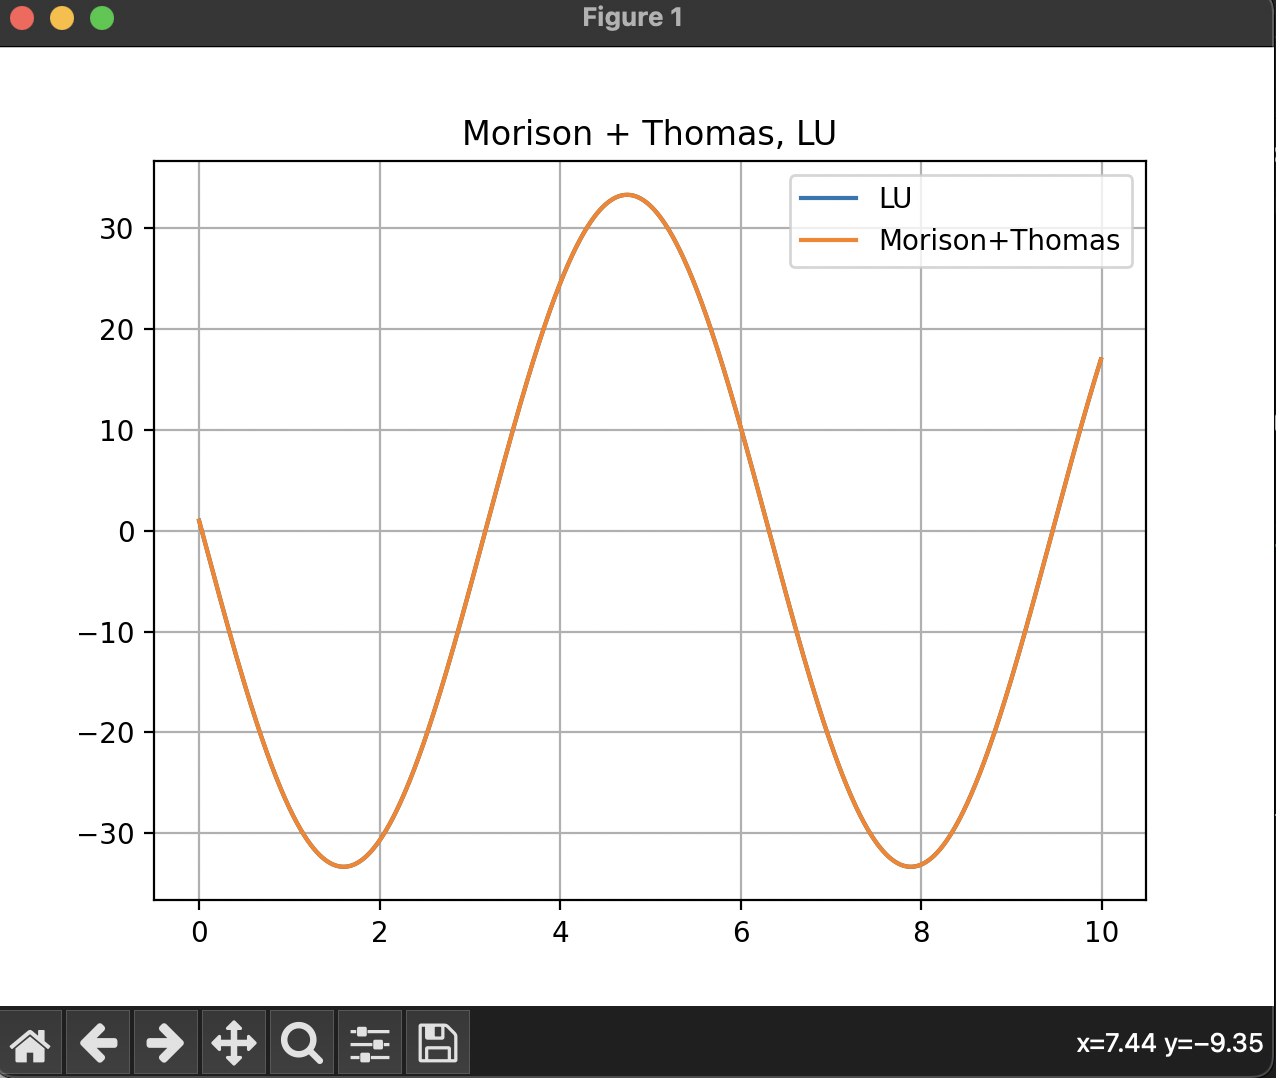
\includegraphics[width=15cm,height=10cm, keepaspectratio]{wykres_sherman}
\subsection{Jawnie:}
\begin{center}
    Czas rozwiazania jawnie: 0.00022292137145996094
    \newline\newline
    Czas rozwazania zwyklym rozkladem LU przy uzyciu numpy: 0.01324009895324707
    \newline\newline
    Wzglednie porównanie LU do morisona: 59.39358288770053
\end{center}
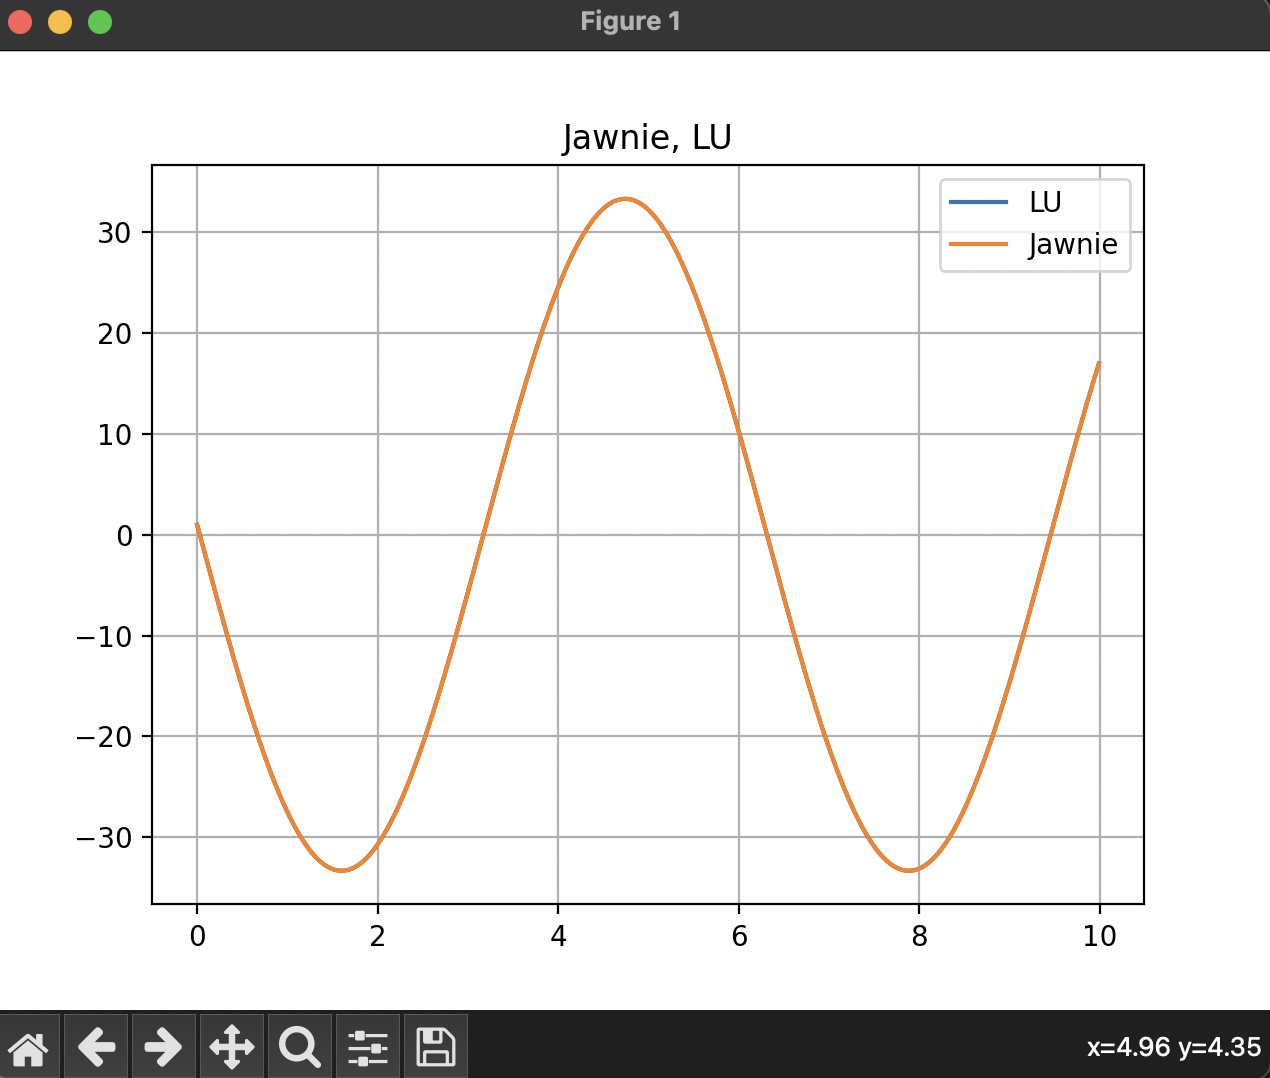
\includegraphics[width=15cm,height=10cm, keepaspectratio]{wykres_jawnie}
\end{document}